\textbf{{算法一:慢开始算法的原理}}

\textbf{{步骤一:~}}在主机刚刚开始发送报文段时可先设置拥塞窗口cwnd=1,\textbf{即设置为一个最大报文段MSS的数值;}

\textbf{{步骤二:}}在每收到一个对新的报文段的确认后,将拥塞窗口加1,即增加一个MSS的数值;

\textbf{{步骤三:}}用这样的方法逐步增大发送端的拥塞窗口cwnd,可以使分组注入到网络的速率更加合理。

\textbf{{\textbf{{算法二:}}{拥塞避免算法的原理}}}

为防止拥塞窗口cwnd的增长引起网络阻塞,还需要一个状态变量,即慢开始门限ssthresh,其用法如下:

当cwnd\textless{}ssthresh时,使用慢开始算法。

当cwnd\textgreater{}ssthresh时,停止使用慢开始算法,改用拥塞避免算法。

当cwnd=ssthresh时,既可以使用慢开始算法,也可以使用拥塞避免算法。

其中,拥塞避免算法的做法是,\textbf{发送端的拥塞窗口cwnd每经过一个往返时延RTT就增加一个MSS的大小}。通常表现为按线性规律增长。

无论在慢开始阶段还是在拥塞避免阶段,只要发送方判断网络出现拥塞(其根据就是没有按时收到确认),{\textbf{就要把慢开始门限ssthresh设置为出现拥塞时的发送窗口值的一半(但不能小于2)}},然后把拥塞窗口cwnd重新设置为1,执行慢开始算法。这样做的目的就是要迅速减少主机发送到网络中的分组数,使得发生拥塞的路由器有足够时间把队列中积压的分组处理完毕。

\textbf{{\textbf{{算法三:}}{快重传算法}}}

首先要求接收方每收到一个失序的报文段后就立即发出重复确认。这样做可以让发送方及早知道有报文段没有到达接收方。发送方只要连续收到3个重复确认就应当立即重传对方尚未收到的报文段。

\textbf{{\textbf{{算法四:}}{快恢复算法}}}

\textbf{{步骤一:}}当发送端{\textbf{收到连续3个重复的确认时}},就执行``乘法减小''算法,把慢开始门限ssthresh设置为当前拥塞窗口的一半。但接下去不执行慢开始算法;

\textbf{{步骤二:}}由于发送方现在认为网络很可能没有发生拥塞,所以现在不执行慢开始算法,即拥塞窗口cwnd现在不设置为1,而是将慢开始门限ssthresh设置为当前拥塞窗口的一半,然后开始执行拥塞避免算法(``加法增大''),使得拥塞窗口缓慢地线性增大,如下图所示;

\textbf{{步骤三:}}若发送窗口值还允许发送报文段,就按拥塞避免算法继续发送报文段。

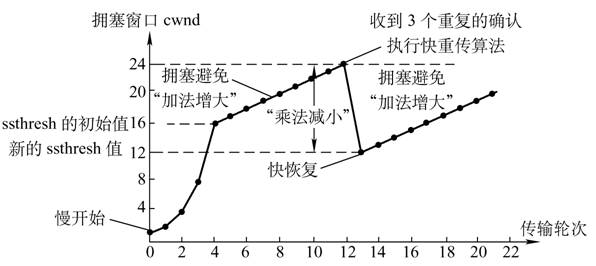
\includegraphics[width=3.43750in,height=1.53125in]{png-jpeg-pics/80404D4E0CFC98A93C39369F240C45EE.png}
